%%=====================================
%% Introduction to Arduino Programming
%% B. Li               Dept of Bioegineering
%% C. Rowlands         Dept of Bioegineering
%% March, 2022
%%=====================================
% first delivery on 23/03/2022

%% compiled in XeLaTeX with Tex Live version 2022.

%% This work is licensed under a Creative Commons Attribution-NonCommercial 4.0 International License.

\documentclass{article}

% margin and font
\usepackage[top=2cm, left=2cm, right=2cm, bottom=1.8cm]{geometry}
\usepackage[utf8]{inputenc}
\usepackage[sfdefault]{arimo}
\usepackage[T1]{fontenc}
% math packages
\usepackage{amsmath}
\usepackage{amsfonts}
\usepackage{mathrsfs} 
\usepackage{mathtools} 
\usepackage{amssymb}
\usepackage{siunitx}
% enable 'resume' function in enumeration
\usepackage{enumitem} 
% graph insertion and float position
\usepackage{graphicx}
\usepackage{float}
% framed text
\usepackage{framed}
% color setting, define hyperref color
\usepackage{xcolor}
\definecolor{linkcolour}{rgb}{0,0.2,0.6}
% hyperref, metadata
\usepackage{hyperref}
\hypersetup{pdfauthor={Li, Binghuan}}
\hypersetup{colorlinks,breaklinks,urlcolor=linkcolour, linkcolor=linkcolour}
% header and footer 
\usepackage{fancyhdr}
\pagestyle{fancy}
\fancyhf{}
\rhead{\thepage}
% appendix section 
\usepackage[title]{appendix}
% tcolorbox
\usepackage[most]{tcolorbox}

% code listing settings
\usepackage{listings}

\lstset{%
  language = C,
  backgroundcolor=\color{white},   
  basicstyle=\footnotesize\ttfamily,       
  breakatwhitespace=false,         
  breaklines=true,                 
  captionpos=b,                   
  commentstyle=\color{gray},    
  deletekeywords={...},           
  escapeinside={\%*}{*)},          
  extendedchars=true,              
  frame=single,                    
  keepspaces=true,                 
  keywordstyle=\color{orange},       
  morekeywords={*,...},            
  numbers=left,                    
  numbersep=5pt,                   
  numberstyle=\footnotesize\color{gray}, 
  rulecolor=\color{black},         
  rulesepcolor=\color{blue},
  showspaces=false,                
  showstringspaces=false,          
  showtabs=false,                  
  stepnumber=2,                    
  stringstyle=\color{orange},    
  tabsize=2,                       
  title=\lstname,
  emphstyle=\bfseries\color{blue}%  style for emph={} 
} 

%% language specific settings:
\lstdefinestyle{Arduino}{
    language = C,
    keywords={void, int boolean},   %  define keywords
    morecomment=[l]{//},            %  treat // as comments
    morecomment=[s]{/*}{*/},        %  define /* ... */ comments
    emph={HIGH, OUTPUT, LOW}        %  keywords to emphasize
}

%%=====================================
\title{Introduction to Arduino Programming}
\author{Binghuan W Li\\ \href{mailto:binghuan.li19@imperial.ac.uk}{\texttt{binghuan.li19@imperial.ac.uk}} \and Dr Christopher Rowlands \\ \href{mailto:c.rowlands@imperial.ac.uk}{\texttt{c.rowlands@imperial.ac.uk}} }
\date{\today}
%%=====================================
\begin{document}

\maketitle
%%=====================================
\section{Introduction}
Today, we will delve a bit into Arduino programming. Originating from Italy, Arduino is an open-source\footnote{The schematics of every board are available to view. You are free to make you own Arduino using standalone components - but you still need to buy them!} electronics prototyping platform based on flexible, easy-to-use hardware and software. It builds on the idea of \textit{using less expensive devices for controlling interactive electronic projects}, supporting rapid prototyping of microcontroller hardware by electronic designers and students. Typically, an Arduino (Nano, Uno) consists a +3.3V power rail, a +5V power rail and two ground(GND) terminals, which can be used to power up most small pieces of external hardware (say, sensors or motors). It also has multiple analogue(A) and digital (D) input/output terminals, which can efficiently control the I/O of your device using signals that you can program youself.\\\\ A detailed pinout of an Arduino Uno is shown below, but more details can be found in the datasheet, available at  \href{https://docs.arduino.cc/static/a106feb536867b39ee791cbc8853b33e/A000066-datasheet.pdf}{here}.
\begin{figure}[H]
    \centering
    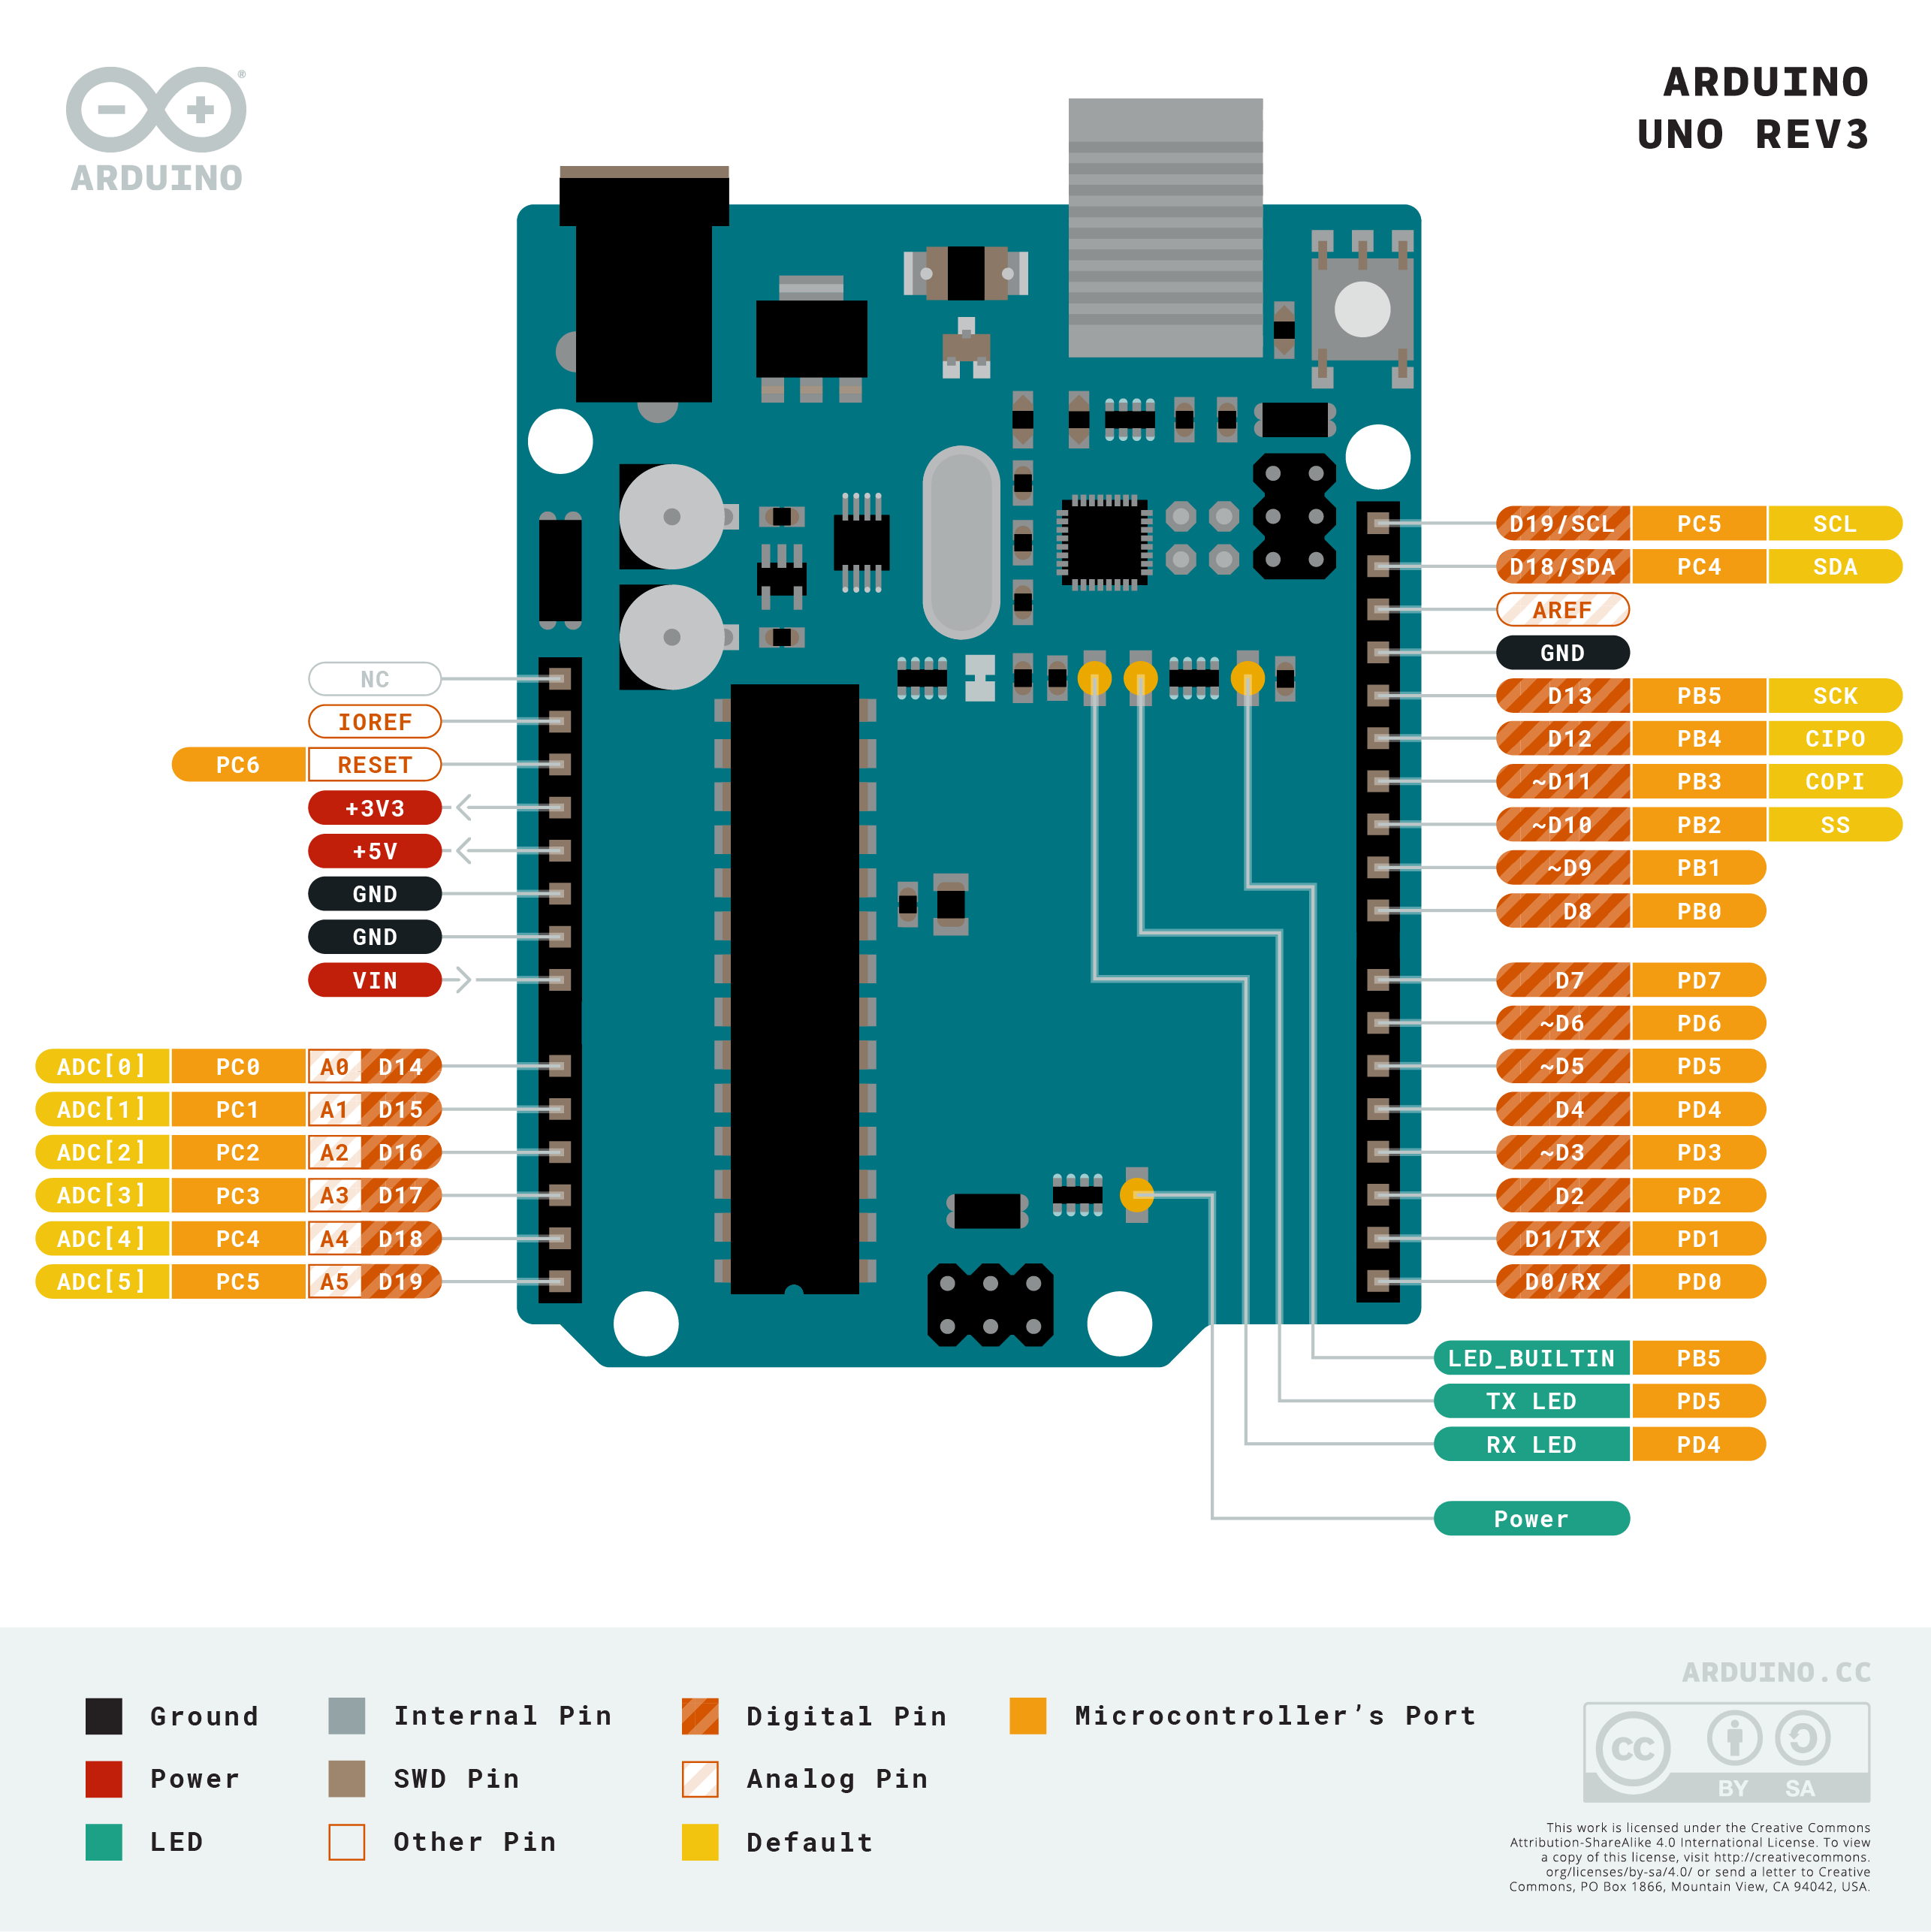
\includegraphics[width=.65\textwidth]{A000066-pinout.png}
    \caption{Arduino Uno pinouts. Adopted from \href{https://content.arduino.cc/assets/Pinout-UNOrev3_latest.png}{https://content.arduino.cc/assets/Pinout-UNOrev3\_latest.png}}
    \label{fig:pinouts}
\end{figure}

%%=====================================
\newpage
\section{From \texttt{Blink} to Arduino Programming Syntax}
\subsection{Arduino IDE}
So, how can you communicate with your Arduino board? Luckily, a `ferry boat', the Arduino IDE, is already there for you, to help you bridge the gap between your computer and the board. Arduino IDE is an integrated development environment introduced by Arduino official, \href{https://www.arduino.cc/en/software}{multiple versions} are available to download for both PC and Mac users. Of course, you are required to write your program in a syntax that is specially designed for Arduino - your Arduino code, or \textbf{sketches}, are written in a variant of C++ called the Arduino Programming Language.\\\\
Once you have installed Arduino IDE successfully on your PC/Mac, the following graphical user interface should be available to you. 
\begin{figure}[H]
    \centering
    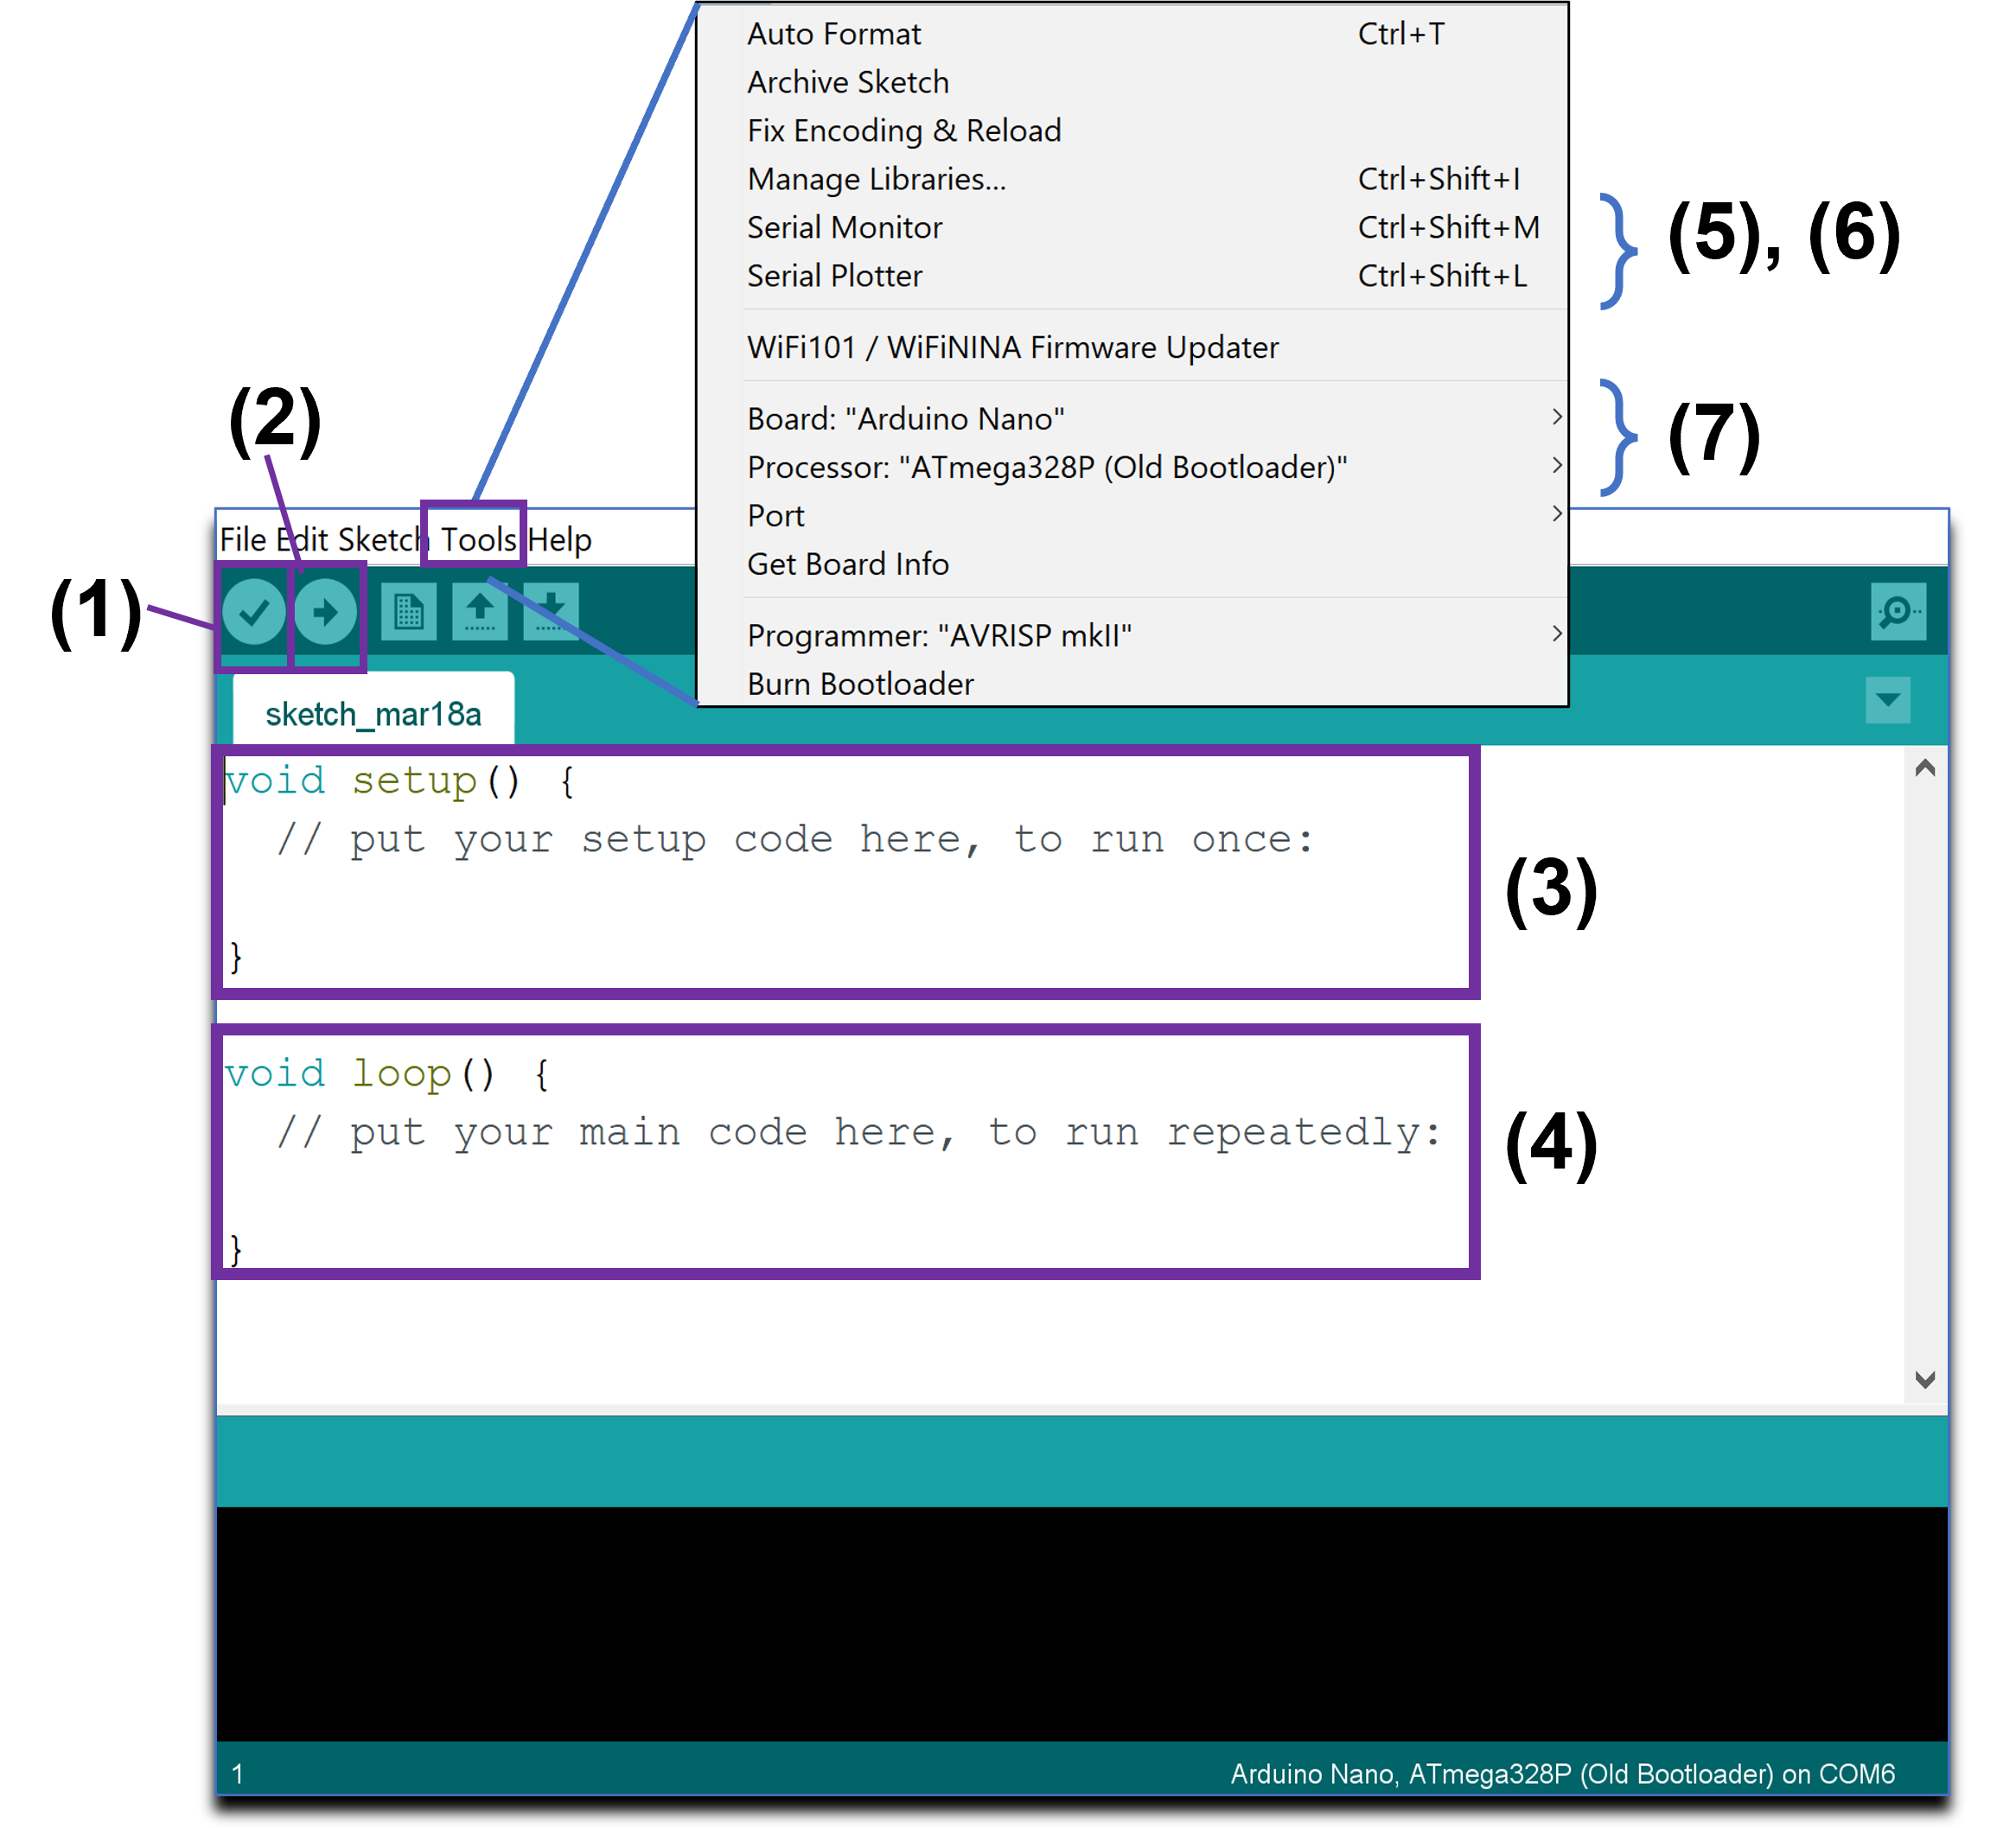
\includegraphics[width=.65\textwidth]{arduino_ide.png}
    \caption{Arduino IDE user interface}
    \label{fig:ide}
\end{figure}
\begin{enumerate}
    \item \textbf{Verify}: by clicking this button, Arduino IDE checks the code for errors, then compiles it, ready for uploading to the Arduino. Click this first.
    \item \textbf{Upload}:  when you click this button, Arduino IDE uploads the code to the connected Arduino board.
    \item \textbf{\texttt{void setup}}: in an Arduino program, statements within this function will only be executed once. Therefore, this function block is commonly used to set up system parameters, etc.
    \item \textbf{\texttt{void loop}}: in an Arduino program, statements within this function will be executed  periodically, similar to if the statements were placed in a \texttt{while True} loop. 
    \item \textbf{Serial monitor}: similar to the console in Python IDLE's IDE, the serial monitor is the `tether' between the computer and your Arduino. It allows you send and receive text messages, handy for debugging and also controlling the Arduino from a keyboard. Unlike the console however, your program needs to be programmed to know how to respond to your text messages!
    \item \textbf{Serial plotter}: similar to the oscilloscopes you've used in the electronics labs, the serial plotter is commonly used to display the data read from the Arduino board. It receives the data (e.g. temperature, humidity) from the hardware sensors and plots the data as one or more waveforms.  
    \item \textbf{Board/processor/port selection}: these options are used to select board model, microcontrollers (by default, ATMega328P) and communication ports in your Arduino IDE. Make sure they match the board you connected to your computer. \textbf{Check these settings every time you connect your Arduino board to your computer.}
\end{enumerate}

\subsection{Blink!} \label{blink}
Similar to \texttt{print("Hello, world!")} in Python and other programming languages, \texttt{Blink} is a very basic Arduino sketch for testing purposes, and to get new learners quickly familiarized with Arduino programming. \\\\This program blinks the on-board light-emitting diode (LED), as well as the LED that is externally connected to digital output pin 13 (if there is one!), with a fixed period of one blink every 2 seconds.
\begin{lstlisting}[label={list:first}, style=Arduino, caption=Blink.ino]
/*
  Blink
  Turns on an LED on for one second, then off for one second, repeatedly.

  Most Arduinos have an on-board LED you can control. On the Uno and
  Leonardo, it is attached to digital pin 13. If you're unsure what
  pin the on-board LED is connected to on your Arduino model, check
  the documentation at http://arduino.cc

  This example code is in the public domain.

  modified 8 May 2014
  by Scott Fitzgerald
 */


// the setup function runs once when you press reset or power the board
void setup() {
  // initialize digital pin 13 as an output.
  pinMode(13, OUTPUT);
}

// the loop function runs over and over again forever
void loop() {
  digitalWrite(13, HIGH);   // turn the LED on (HIGH is the voltage level)
  delay(1000);              // wait for a second
  digitalWrite(13, LOW);    // turn the LED off by making the voltage LOW
  delay(1000);              // wait for a second
}
\end{lstlisting}
\noindent The corresponding wiring schematic is shown below. The resistor, $R=220\Omega$.
\begin{figure}[H]
    \centering
    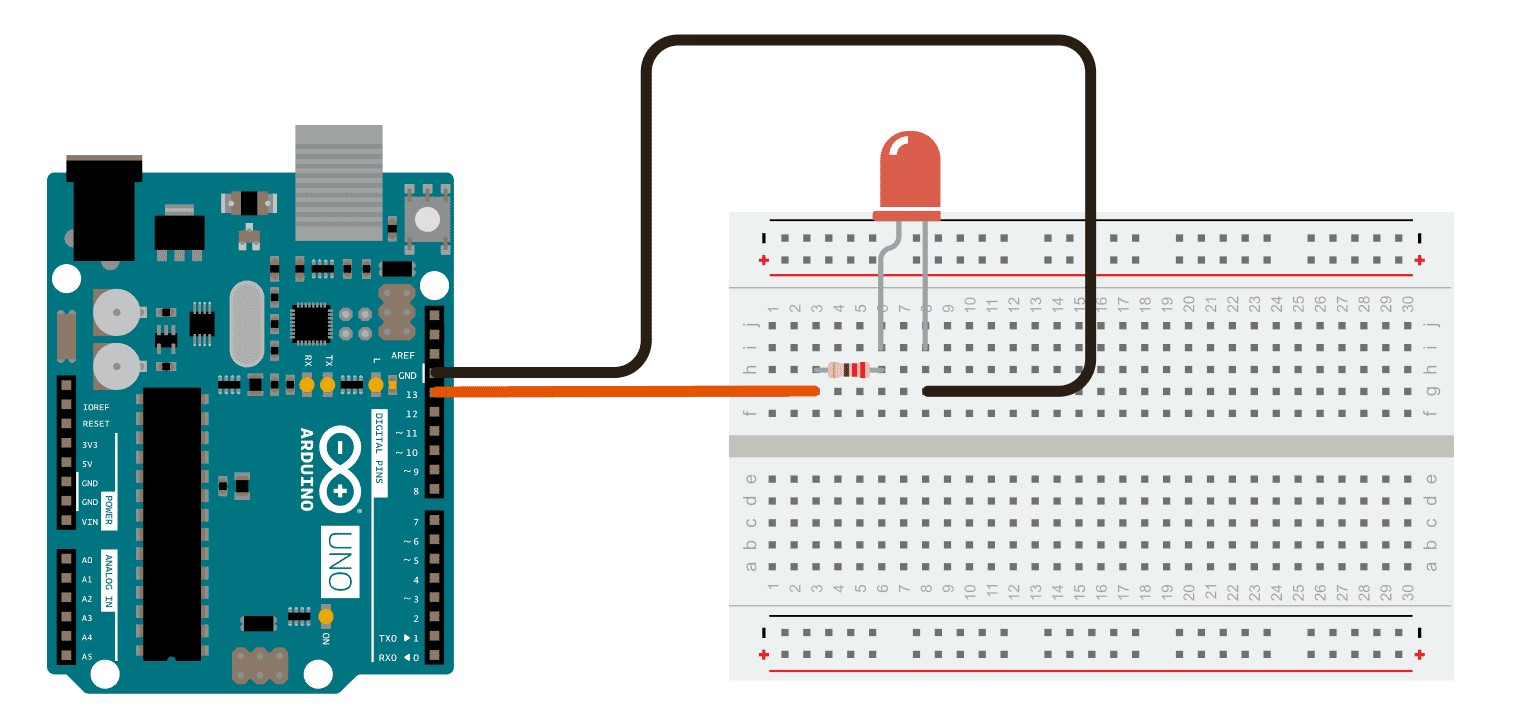
\includegraphics[width=.6\textwidth]{blink.jpg}
    \caption{Schematic for Blink}
    \label{fig:blink}
\end{figure}

\begin{tcolorbox}[breakable]
\noindent A detailed code breakdown: 
\begin{enumerate}
    \item \texttt{void setup()} - \texttt{setup} is the name of the function which runs once, whenever the board is turned on (or reset). \texttt{void} means it returns no varaiables, and the empty brackets mean that it takes no arguments. Statements within this function will only be executed once.\\\\ In C++/C-like programming languages, when returning a value from a function, you are required to tell your compiler what data type that value is (such as \texttt{int}, \texttt{char}, \texttt{float}, or any other data type). In this case, the return type is \texttt{void}, which just tells the compiler that there is no return value.
    
    \item \texttt{pinMode(13, OUTPUT)} - this command initializes pin 13 on your Arduino board as an output pin. \\\\The general format of this command is \texttt{pinMode(pin, mode)}; it takes two arguments, which specify the \texttt{mode} (\texttt{OUTPUT} or \texttt{INPUT}) of a specific pin.
    
    \item \texttt{void loop()} - similar to \texttt{void setup()}, the function \texttt{loop} does not return any value. Statements within this function will be executed periodically while the board is active.
    
    \item \texttt{digitalWrite(13, HIGH)} - this command controls your Arduino board, telling it to turn the LED on by supplying a +5V voltage ($V_{cc}$) to pin 13 (and thus to the anode of your LED). The same is true for \texttt{digitalWrite(13, LOW)}, which will turn off the LED, taking the voltage supply back to 0V.
    
    \item \texttt{delay(1000)} - this command tells the board to do nothing for 1000 milliseconds, or 1 second. It is similar to the \texttt{time.sleep} function in Python.
\end{enumerate}
Other general comments on coding syntax:
\begin{enumerate}[resume]
    \item \textbf{Semicolons} - In Arduino sketches or C++/C-like programming languages, a semicolon \textbf{\large ;} is required to end your statements. Usage of Semicolons in C will remove ambiguity and confusion while looking at the code. However, this is optional in Python.
    
    \item \textbf{Comments} - In Arduino sketches or C++/C-like programming languages, \textbf{multiline comments} are inserted between \textbf{\large /*...*/} while \textbf{single line comments} are inserted after double backslashes \textbf{\large //}. Comments will be ignored by the compiler. 
\end{enumerate}
\end{tcolorbox}


\subsection{Variables and Arithmetic Expressions}
In this section, we are going to see the different data types and operators that you may find useful in your sketches. The following syntax can also be applied to other C-like languages, including C and C++.
\subsubsection{Variable declaration}
In all C-like programming languages, variables must be \textbf{declared} before they are used. A declaration consists of a \textit{type name} and \textit{variable(s)}. You can assign a value to the variable right after you declare it. For example:
\begin{lstlisting}
int my_variable_1 = 25; \\ declare an integer type variable, assign a value to it.
char greeting[6] = {'H', 'e', 'l', 'l', 'o', '\0'}; \\ strings are terminate by \0.
\end{lstlisting}\vspace{-.5cm}
Primary data types include \texttt{int} (integer, 16 bits),  \texttt{float}(floating point, 32 bits), \texttt{char}(character, 8 bits), \texttt{double}(double precision floating point) etc. \\\\Moreover, \textbf{modifiers} - \texttt{signed}, \texttt{unsigned}, \texttt{short}, and \texttt{long} are used to modify default properties of primary data types. For example, by applying \texttt{unsigned} modifier to the \texttt{int} type, the variable can only store values greater than or equal to zero.\\\\A clear and neat summary of C data types in a table can be found \href{https://en.wikipedia.org/wiki/C_data_types}{here}. A  `friendly' explanation to C data types and modifiers can be found \href{https://www.journaldev.com/26779/data-types-and-modifiers-in-c}{here}. 

\subsubsection{Arithmetic expressions}
A large set of operators are available in the Arduino Programming Language. Here are a few quick cheat sheets you can use in your Arduino programming.
\begin{table}[H]
    \centering
    \begin{tabular}{c|c||c|c} \hline
        Operator & Meaning & operator & Meaning\\ \hline
        + & addition & - & subtraction \\
        * & multiplication & / & division \\
        \% & reminder after division & & \\\hline
    \end{tabular}
    \caption{Arithmetic operators}
\end{table}
\begin{table}[H] \vspace{-.5cm}
    \centering
    \begin{tabular}{c|c||c|c} \hline
        Operator & Meaning & operator & Meaning\\ \hline
        = & a=b & += & a+=b equivalent to a=a+b \\
        -= & a-=b equivalent to a=a-b & *= & a*=b equivalent to a=a*b \\
        /= & a/=b equivalent to a=a/b & \%= & a\%=b equivalent to a=a\%b \\\hline
    \end{tabular}
    \caption{Assignment operators}
\end{table}
\begin{table}[H]\vspace{-.5cm}
    \centering
    \begin{tabular}{c|c||c|c} \hline
        Operator & Meaning & operator & Meaning\\ \hline
        == & equal to, 	\textit{e.g.} \texttt{5==3}$\Rightarrow$0 & > & greater than \\
        < & smaller than & != & not equal to \\
        >= & greater than or equal to & <= & less than or equal to \\\hline
    \end{tabular}
    \caption{Relational operators}
\end{table}
\begin{table}[H]\vspace{-.5cm}
    \centering
    \begin{tabular}{c|c} \hline
        Operator & Meaning\\ \hline
        \&\& & Logical AND. True only if all operands are true  \\
        || & Logical OR. True only if either one operand is true \\
        ! & Logical NOT. True only if the operand is 0 \\\hline
    \end{tabular}
    \caption{Logical operators}
\end{table}

\subsection{Control flow}
In this section, we will look at the syntax of common control flow constructs - \texttt{for} loops, \texttt{if...else...} statements and \texttt{while} loops.\\\\
While we are only covering these three control flow statements here, note that there are more useful statements supported by C-like languages: \href{https://www.programiz.com/c-programming/c-do-while-loops}{\texttt{do...while}} loops, \href{https://www.programiz.com/c-programming/c-switch-case-statement}{\texttt{switch}} case, \href{https://www.programiz.com/c-programming/c-break-continue-statement}{\texttt{break} and \texttt{continue}} statements.

\subsubsection{\texttt{for} loop}
\begin{minipage}{.6\textwidth}
\texttt{for} loops in Arduino sketches are following the structure below - three arguments are given in the order of initial condition-final condition-action, as shown in the parenthesis following the keyword \texttt{for}. \\\\A quick example is \texttt{for(int i=0, i<=5, i++)}.
\begin{lstlisting}[caption=for loop]
for (initial_condition, final_condition, action){
    statement_1;
    statement_2;
    ...
}
\end{lstlisting}
\end{minipage}\hfill
\begin{minipage}{.35\textwidth} 
\begin{figure}[H]\vspace{-1cm}
    \centering
    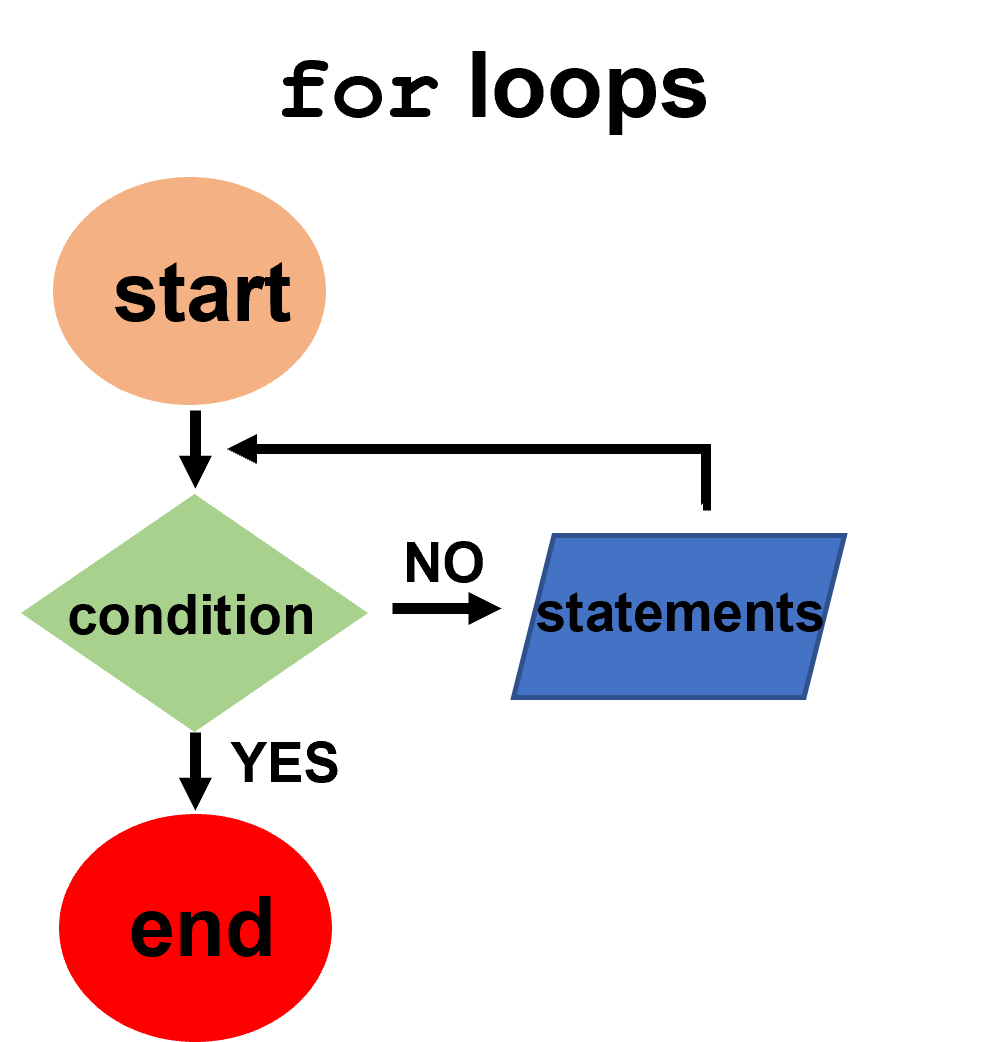
\includegraphics[width=.75\textwidth]{for_loop.png}
    \caption{\texttt{for} loop}
\end{figure}
\end{minipage}\\\\\\
\noindent Note the differences from Python's \texttt{for} loop syntax : There is no syntactic whitespace. C-like languages place the code within the loop inside of two curly brackets {}. It is however very good practice to still indent the statements in the loop, so you can read the code more easily. Don't forget you still need a semicolon at the end of each statement in the loop!

\subsubsection{\texttt{if...else...}statements}
\begin{minipage}{.6\textwidth}
\texttt{if...else-if...else...} statements in Arduino sketches share a very similar syntax to Python, except \texttt{elif} in Python is written as \texttt{else if} in an Arduino sketch. \vspace{.2cm}
\begin{lstlisting}[caption=if else statements]
if (condition_1){
    statement_block_1;
}
else if (condition_2){
    statement_block_2;
}
else{
    statement_block_3;
}
\end{lstlisting}
\end{minipage}\hfill
\begin{minipage}{.35\textwidth}
\begin{figure}[H]\vspace{-1cm}
    \centering
    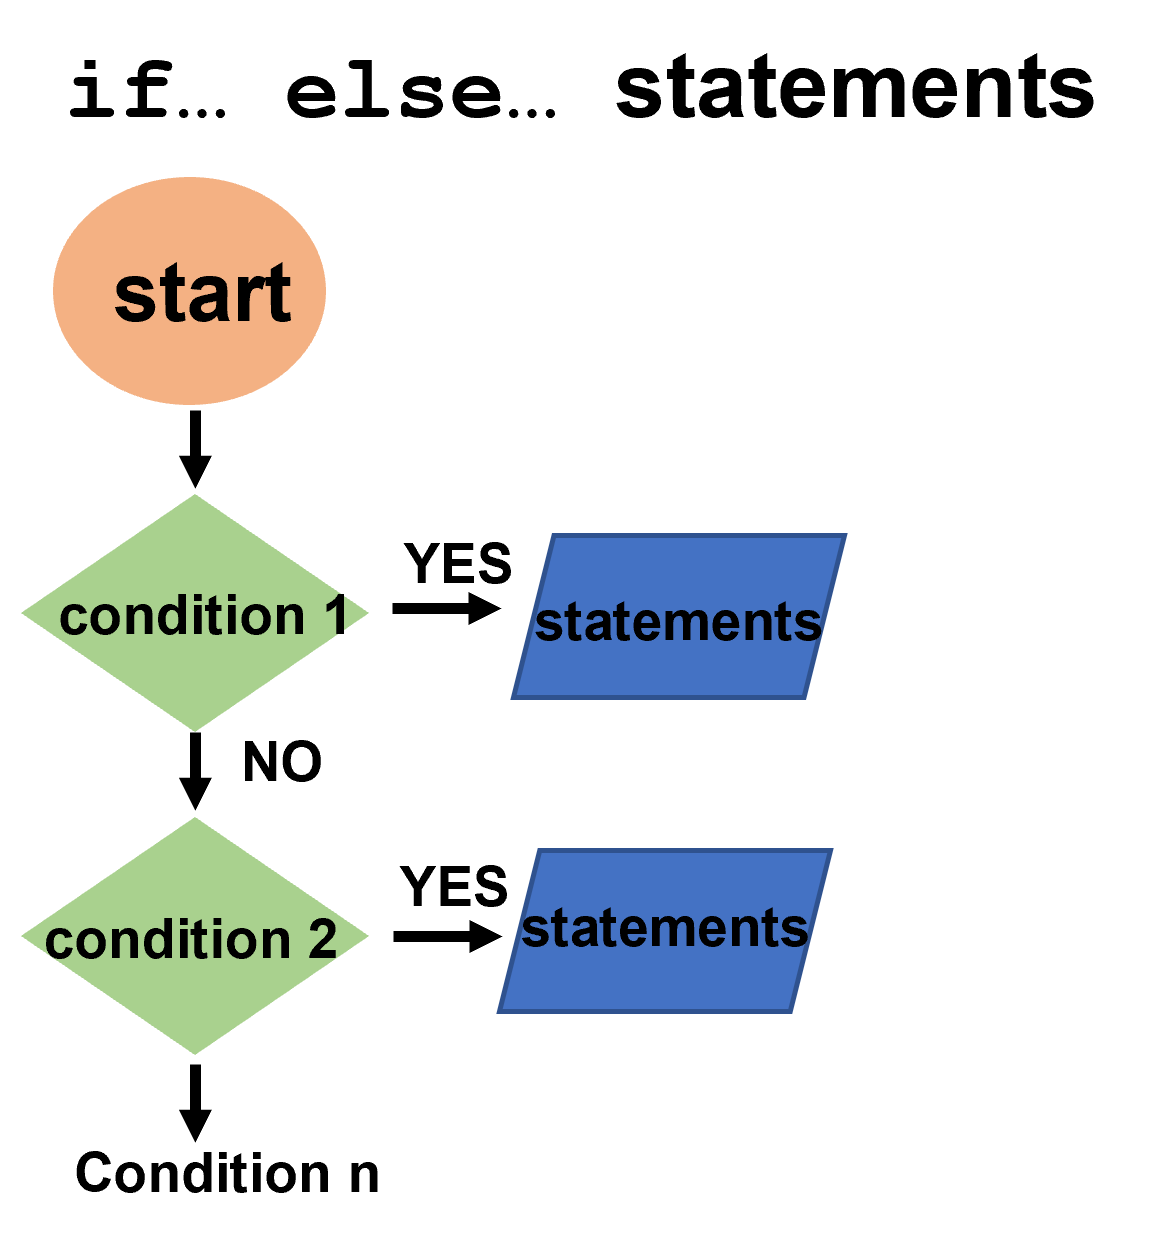
\includegraphics[width=.75\textwidth]{ifelse.png}
    \caption{\texttt{if... else...} statements}
\end{figure}
\end{minipage}

\subsubsection{\texttt{while} loop}
\begin{minipage}{.6\textwidth}
\texttt{while} loops in Arduino sketches also share a similar syntax to those in Python. In a \texttt{while} loop, a condition check is given in the parentheses, statements are expressed between the curly brackets. The while loop will execute so long as the condition check evaluates to \texttt{true}; the check will be performed each time the loop repeats, so make sure it will evaluate to \texttt{false} at some point or your program will get stuck! \vspace{.2cm}
\begin{lstlisting}[caption=while loop]
while (true_condition){
    statement_1;
    statement_2;
    ...
    statement_increment_to_true_condition;
}
\end{lstlisting}
\end{minipage}\hfill
\begin{minipage}{.35\textwidth}
\begin{figure}[H]\vspace{-1cm}
    \centering
    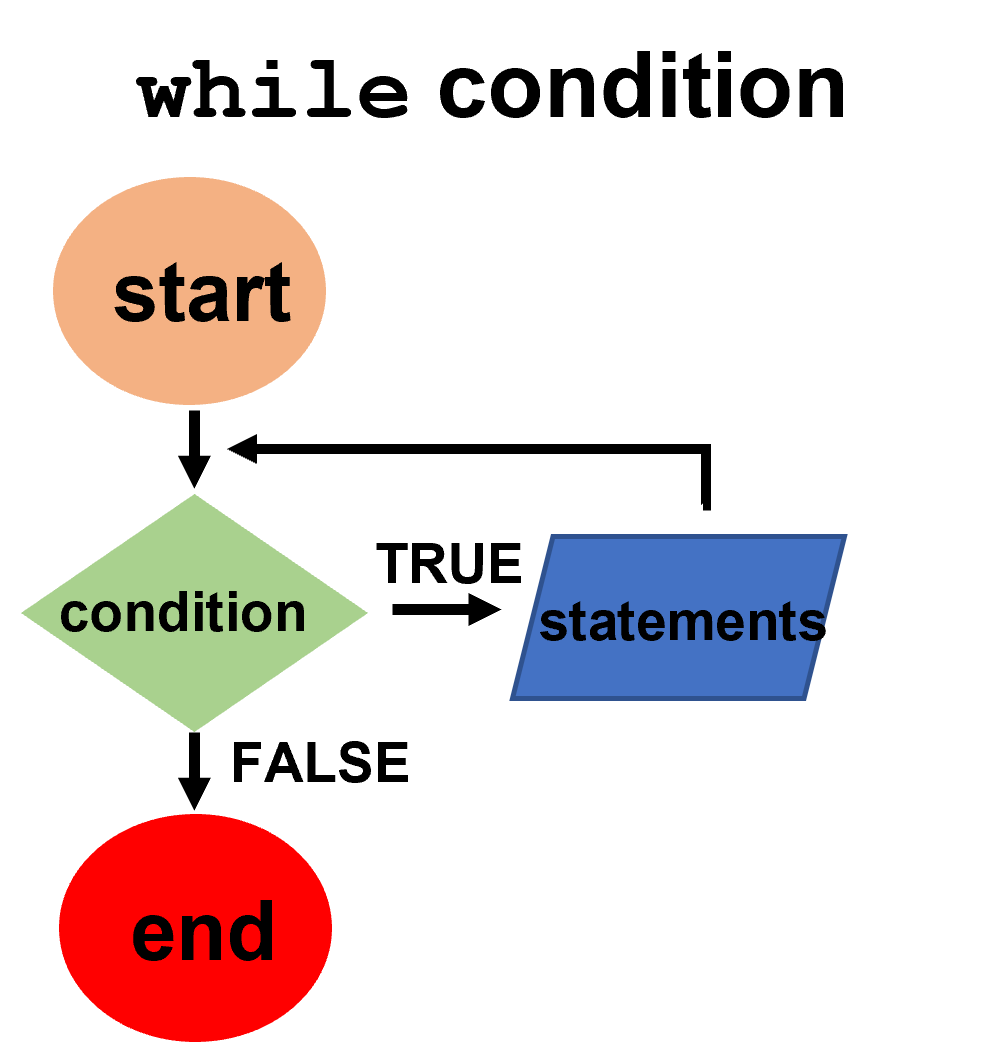
\includegraphics[width=.75\textwidth]{while.png}
    \caption{\texttt{while} loop}
\end{figure}
\end{minipage}


\subsection{Functions}
Like Python, Arduino Programming Language (and, in fact, any C-like language) allows you to define functions. A function definition in an Arduino sketch follows the structure below:
\begin{lstlisting}
return_type function_name (arg1, arg2, ..., argN) {
    statement_1;
    statement_2;
    ...
    statement_N;
    return value;
}
\end{lstlisting}
\vspace{-.5cm}
All functions must have a function return type that is specified prior to the function name. This type can be \texttt{int}, \texttt{float}, \texttt{char*} \footnote{The asterisk declares a pointer. The pointer stores the starting memory location of the variable it is next to, in this case a string.} or simply \texttt{void} (return nothing). \\\\The function name and arguments come after the return type, and at this point there is fundamentally nothing different from Python's function definition. As before however, there is no syntactic white space; all statements should be placed in between the curly brackets. Although indentation is not compulsory in C-like languages, they improve your code readability - you should definitely use it.\\\\ A \texttt{return} statement is used to return values/variables from the function. It is optional. Sometimes, even there is no need to return any variables from the function, people use  \texttt{return 0} to indicate that the function executed correctly, and use non-zero returns (e.g, \texttt{return -1}) to indicate errors.


%%=====================================
\newpage
\section{Serial communication at a glance}
Well, after going through some basic syntax which will be useful in Arduino sketches (ah, finally!), you are now a shining expert in Arduino coding! Wait... you may ask, are there any specific features for Arduino \textit{only}, but not for other C-like languages? The answer is "yes", and one of the most important features is \href{https://en.wikipedia.org/wiki/Serial_communication}{\textbf{serial communication}}.\\\\
Serial communication is used for data transfer between the Arduino board and your device (let us say, your PC), by sending bite-sized data sequentially over a \textbf{communication port} (COM). This is how your compiled sketch can be uploaded and executed on the board, and is also how the data collected from an external device (let us say, a temperature sensor), can be sent back to your PC.
\begin{figure}[H]
    \centering
    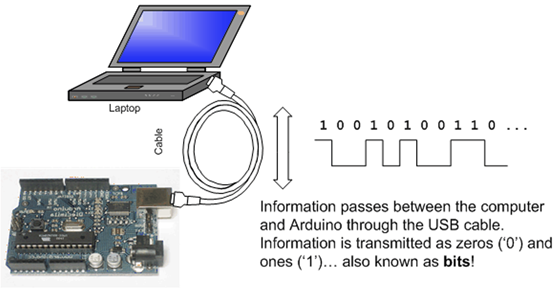
\includegraphics[width=.6\textwidth]{serialdata.png}
    \caption{Serial communication. Adopted from \href{https://www.ladyada.net/learn/arduino/lesson4.html}{https://www.ladyada.net/learn/arduino/lesson4.html}}
\end{figure}
\noindent Look carefully to your Arduino board, there are two helpful built-in LEDs, labeled with RX and TX, that will blink when the Arduino is receiving data (RX) as well as transmitting data (TX). You can use them whenever you are communicating with the board, to check that everything is working properly.\\\\
Now, we are going to look at five useful functions which are related to serial communication. However, this is but a small selection of the functions available; more can be found \href{https://www.arduino.cc/reference/en/language/functions/communication/serial/}{here}.

\subsection{\texttt{Serial.begin()}}
The first function related to the serial communication is \texttt{Serial.begin(\textit{speed})}. This function takes one compulsory argument, \texttt{speed}, which sets the data rate (baud, or bits per second) for serial data transmission. \\\\ By convention, we take the data transmission rate to 9600 baud (i.e. \texttt{Serial.begin(9600)}), as this is the default rate for the Arduino. You should be aware that your Arduino (and other devices) can communicate at different speeds, so make sure you check the manual for whatever you are trying to communicate with.\\\\DO include this command in your \texttt{void setup()} function, as most likely you do not want this command to be executed periodically!

\subsection{\texttt{Serial.print()}}
Similar to Python, the \texttt{print} function is particularly useful to print data to a particular output device. Unlike in your Python code however, we don't have a console to print to, so instead we print to the serial port. This function takes 1 compulsory argument. For example, \texttt{Serial.print(`Hello, world!');} gives `Hello, world!'. \\\\The second argument is optional, it is used to specify the base of the value to print. For example, \texttt{Serial.print(78, BIN);} gives `1001110', as it converts a decimal number into the binary form.

\subsection{\texttt{Serial.println()}}
This function is \textit{almost} identical to \texttt{Serial.print()}, but every time we call this function, it will start with printing with a new line.\\\\How does your program achieve this function...? Basically, an \textbf{escape sequence}, {\texttt{\Large\textbackslash n}}, will be appended to your string, which tells your program to start a new line. You may remember this from the ASCII and Unicode slides in the first lecture of the course.

\subsection{\texttt{Serial.read()}}
The function \texttt{Serial.read()} is used for reading incoming serial data. It does not take any arguments, but returns the first byte of incoming serial data with an \texttt{int} data type. You should notice that this helps explain why in C (and even in Python), variables have a type. The compiler or interpreter knows how to interpret the sequence of 1s and 0s so that they represent what the programmer wants them to represent (a number, or a string, or a boolean for example). Here, we don't know what the data type returned from the serial port is, so we just guess that it is an \texttt{int}. We might be wrong!\\\\Usually, the use of \texttt{Serial.read()} is accompanied with another function \texttt{Serial.available()}, which returns how many bytes of data have arrived in the serial buffer, and therefore are ready to be read. Make sure you don't wait too long before reading from the buffer, as it can overflow and you will lose data!
\begin{lstlisting}
void loop() {
    if (Serial.available() > 0) {
        int incomingByte = Serial.read();
    }
}
\end{lstlisting}
\vspace{-.8cm}
\subsection{\texttt{Serial.write()}}
The final function we are going to analyse is \texttt{Serial.write()}. It writes binary data to the serial port. If the argument is a value, the data will be sent as a byte; if the argument is a string, the it will be sent as a series of bytes. 




%%=====================================
\newpage
\section{Analog? Digital?}
In \autoref{blink}, we had a brief exposure to Arduino digital pins as well as the digital output function \texttt{digitalWrite()}. In this section, we will delve a bit deeper into the digital/analog output/input functions on the Arduino boards. {\color{red} First, to use the functions below, remember to initialize \texttt{pinMode()} in \texttt{void setup()}!} 

\subsection{Analog signals - \texttt{analogRead} and \texttt{analogWrite}}
Arduinos can both input (read) and output (write) analog signals. To \textit{read} an input analog signal, the function \texttt{analogRead(\textit{pin})} is useful; it tells the Arduino's built-in analog-to-digital converter (ADC) to convert an analog signal into a digital value and return an integer between 0 and 1023. This digital value is is proportional to that of a reference voltage, either 5V or 3.3V. You should look up the specifications for the board you are using to know what the reference voltage is.\\\\
To \textit{write} an analog signal, although no digital-to-analog converters (DACs) are pre-built into Arduino Uno or Arduino Nano\footnote{If you need a DAC you can either use a separate DAC chip, or the Arduino Due has two built in.}, Arduinos can \textbf{pulse-width modulate} (PWM) a digital signal to achieve an analog output, through the function \texttt{analogWrite(\textit{pin}, \textit{value})}. This function takes two arguments - the first argument specifies the output pin, the second argument is an integer value between 0 to 255 that is proportional to the \textbf{duty cycle} of the signal. \\\\ 
To illustrate how PWM works in an Arduino board, refer to  \autoref{fig:pwm}. PWM works by very rapidly switching between two states (on and off), spending more time in one state than the other. The signal is then low-pass filtered to get an 'average' value, which will be somewhere between V\textsubscript{on} and V\textsubscript{off}. When value = 0, the signal is always OFF; when value = 255, the signal is always ON. By altering the value, a digital signal can be used to `imitate' an analog signal. To determine the value based on your desired voltage, the following equation is used:
\[value = 51 \times u\]
where $u$ is your desired analog voltage.
\begin{figure}[H]
    \centering
    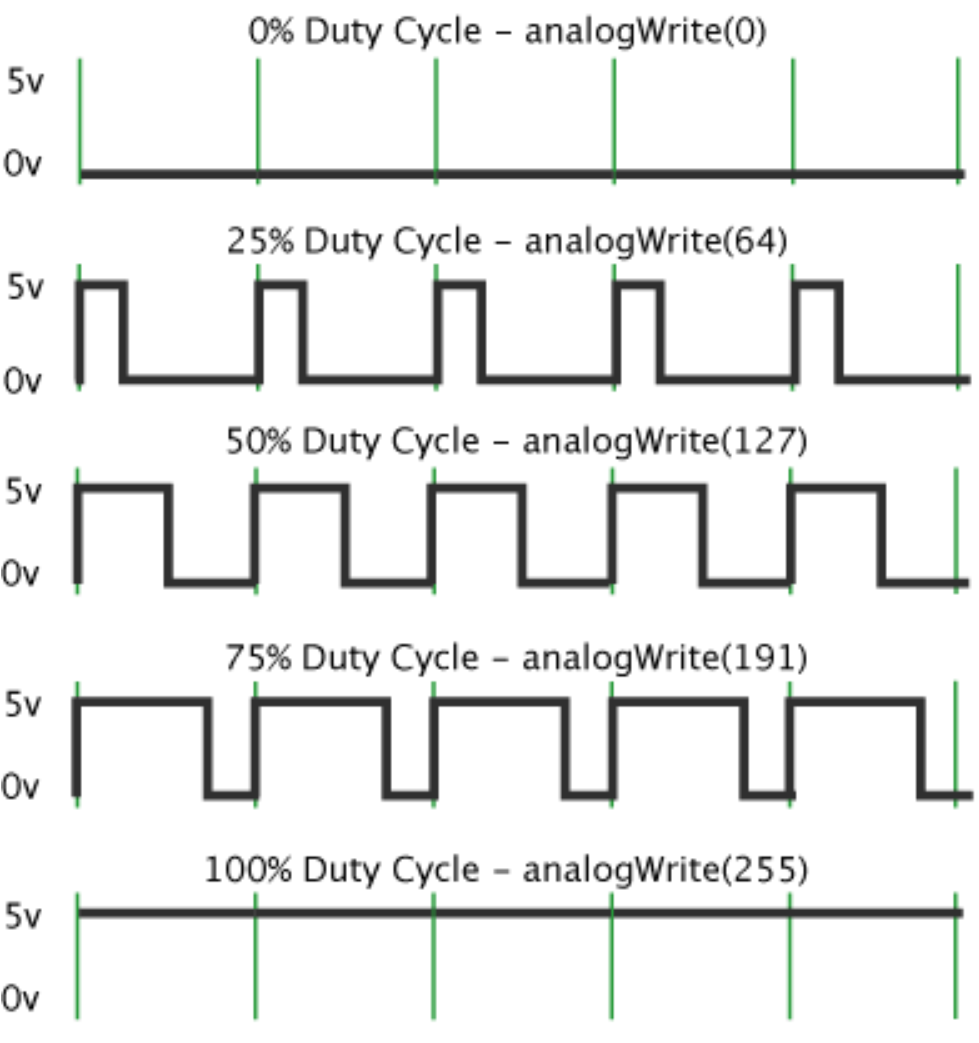
\includegraphics[width=.4\textwidth]{pwm.png}
    \caption{Pulse-width modulation. Adopted from \href{https://www.arduino.cc/en/Tutorial/Foundations/PWM}{https://www.arduino.cc/en/Tutorial/Foundations/PWM}}
    \label{fig:pwm}
\end{figure}
\noindent \textbf{Note: NOT all pins support PWM!} On most Arduino boards, the PWM function is available on pins 3, 5, 6, 9, 10, and 11. The frequency of the PWM signal on most pins is approximately 490 Hz. On the Uno and similar boards, pins 5 and 6 have a frequency of approximately 980 Hz.
\subsection{Digital signals}
Analogous to \texttt{analogRead(\textit{pin})} and \texttt{analogWrite(\textit{pin}, \textit{value})}, there are equivalent functions for digital signals, \texttt{digitalRead(\textit{pin})} and \texttt{digitalWrite(\textit{pin}, \textit{value})}. These perform input and output for digital signals, respectively. There is a minor difference however - the second argument of the function \texttt{digitalWrite(\textit{pin}, \textit{value})} can only take two expressions: `HIGH' or `LOW'.
% \begin{center}\vspace{-.2cm}
%   {\color{red} To use the functions above, remember to initialize \texttt{pinMode()} in \texttt{void setup()}!} 
% \end{center}


%%=====================================
%%=====================================
\newpage
\begin{appendices}

\section{From sketches to actions - compilation}
When you click the `upload' button in your Arduino IDE, an sequence of important events have to happen to pass your sketch to your Arduino board. These events are complicated, but to break them down into a manageable outline, below is a very brief description. Nevertheless, a full, comprehensive explanation can be found \href{https://arduino.github.io/arduino-cli/0.21/sketch-build-process/}{here}.
\begin{enumerate}
    \item \textbf{Pre-processing}: during this stage, your \texttt{.ino} sketches will be processed into a C++ program (\texttt{.cpp}). This step is unique in Arduino Programming Language.
    \item \textbf{Compilation}: at this stage, the C++ program that is obtained from the last step will be compiled into machine-readable instructions by the avr-gcc compiler. \\\\To take a closer look the compilation process: first, an object file (\texttt{.o}) is generated. Your compiler will link\footnote{Linking is when the 'linker' finds all the extra code from the libraries and functions you call in your code, and puts the actual code for those functions into your program} this object file to the standard Arduino libraries. The standard Arduino libraries enable us to use those Arduino built-in functions, such as \texttt{Serial.begin()} and \texttt{digitalWrite()}. \\\\Meanwhile, your compiler will try to locate the dependencies (say, external libraries, \texttt{.h} files) if you have added any \texttt{\#include} statements in your sketch. This process is known as \textbf{separate compilation}. 
    \item \textbf{Uploading}: the final output of the compilation is a \texttt{.hex} file. The \texttt{.hex} file is uploaded to the board by a uploader/downloader utility, Avrdude, over the USB or serial connection.
\end{enumerate}
\begin{figure}[H]
    \centering
    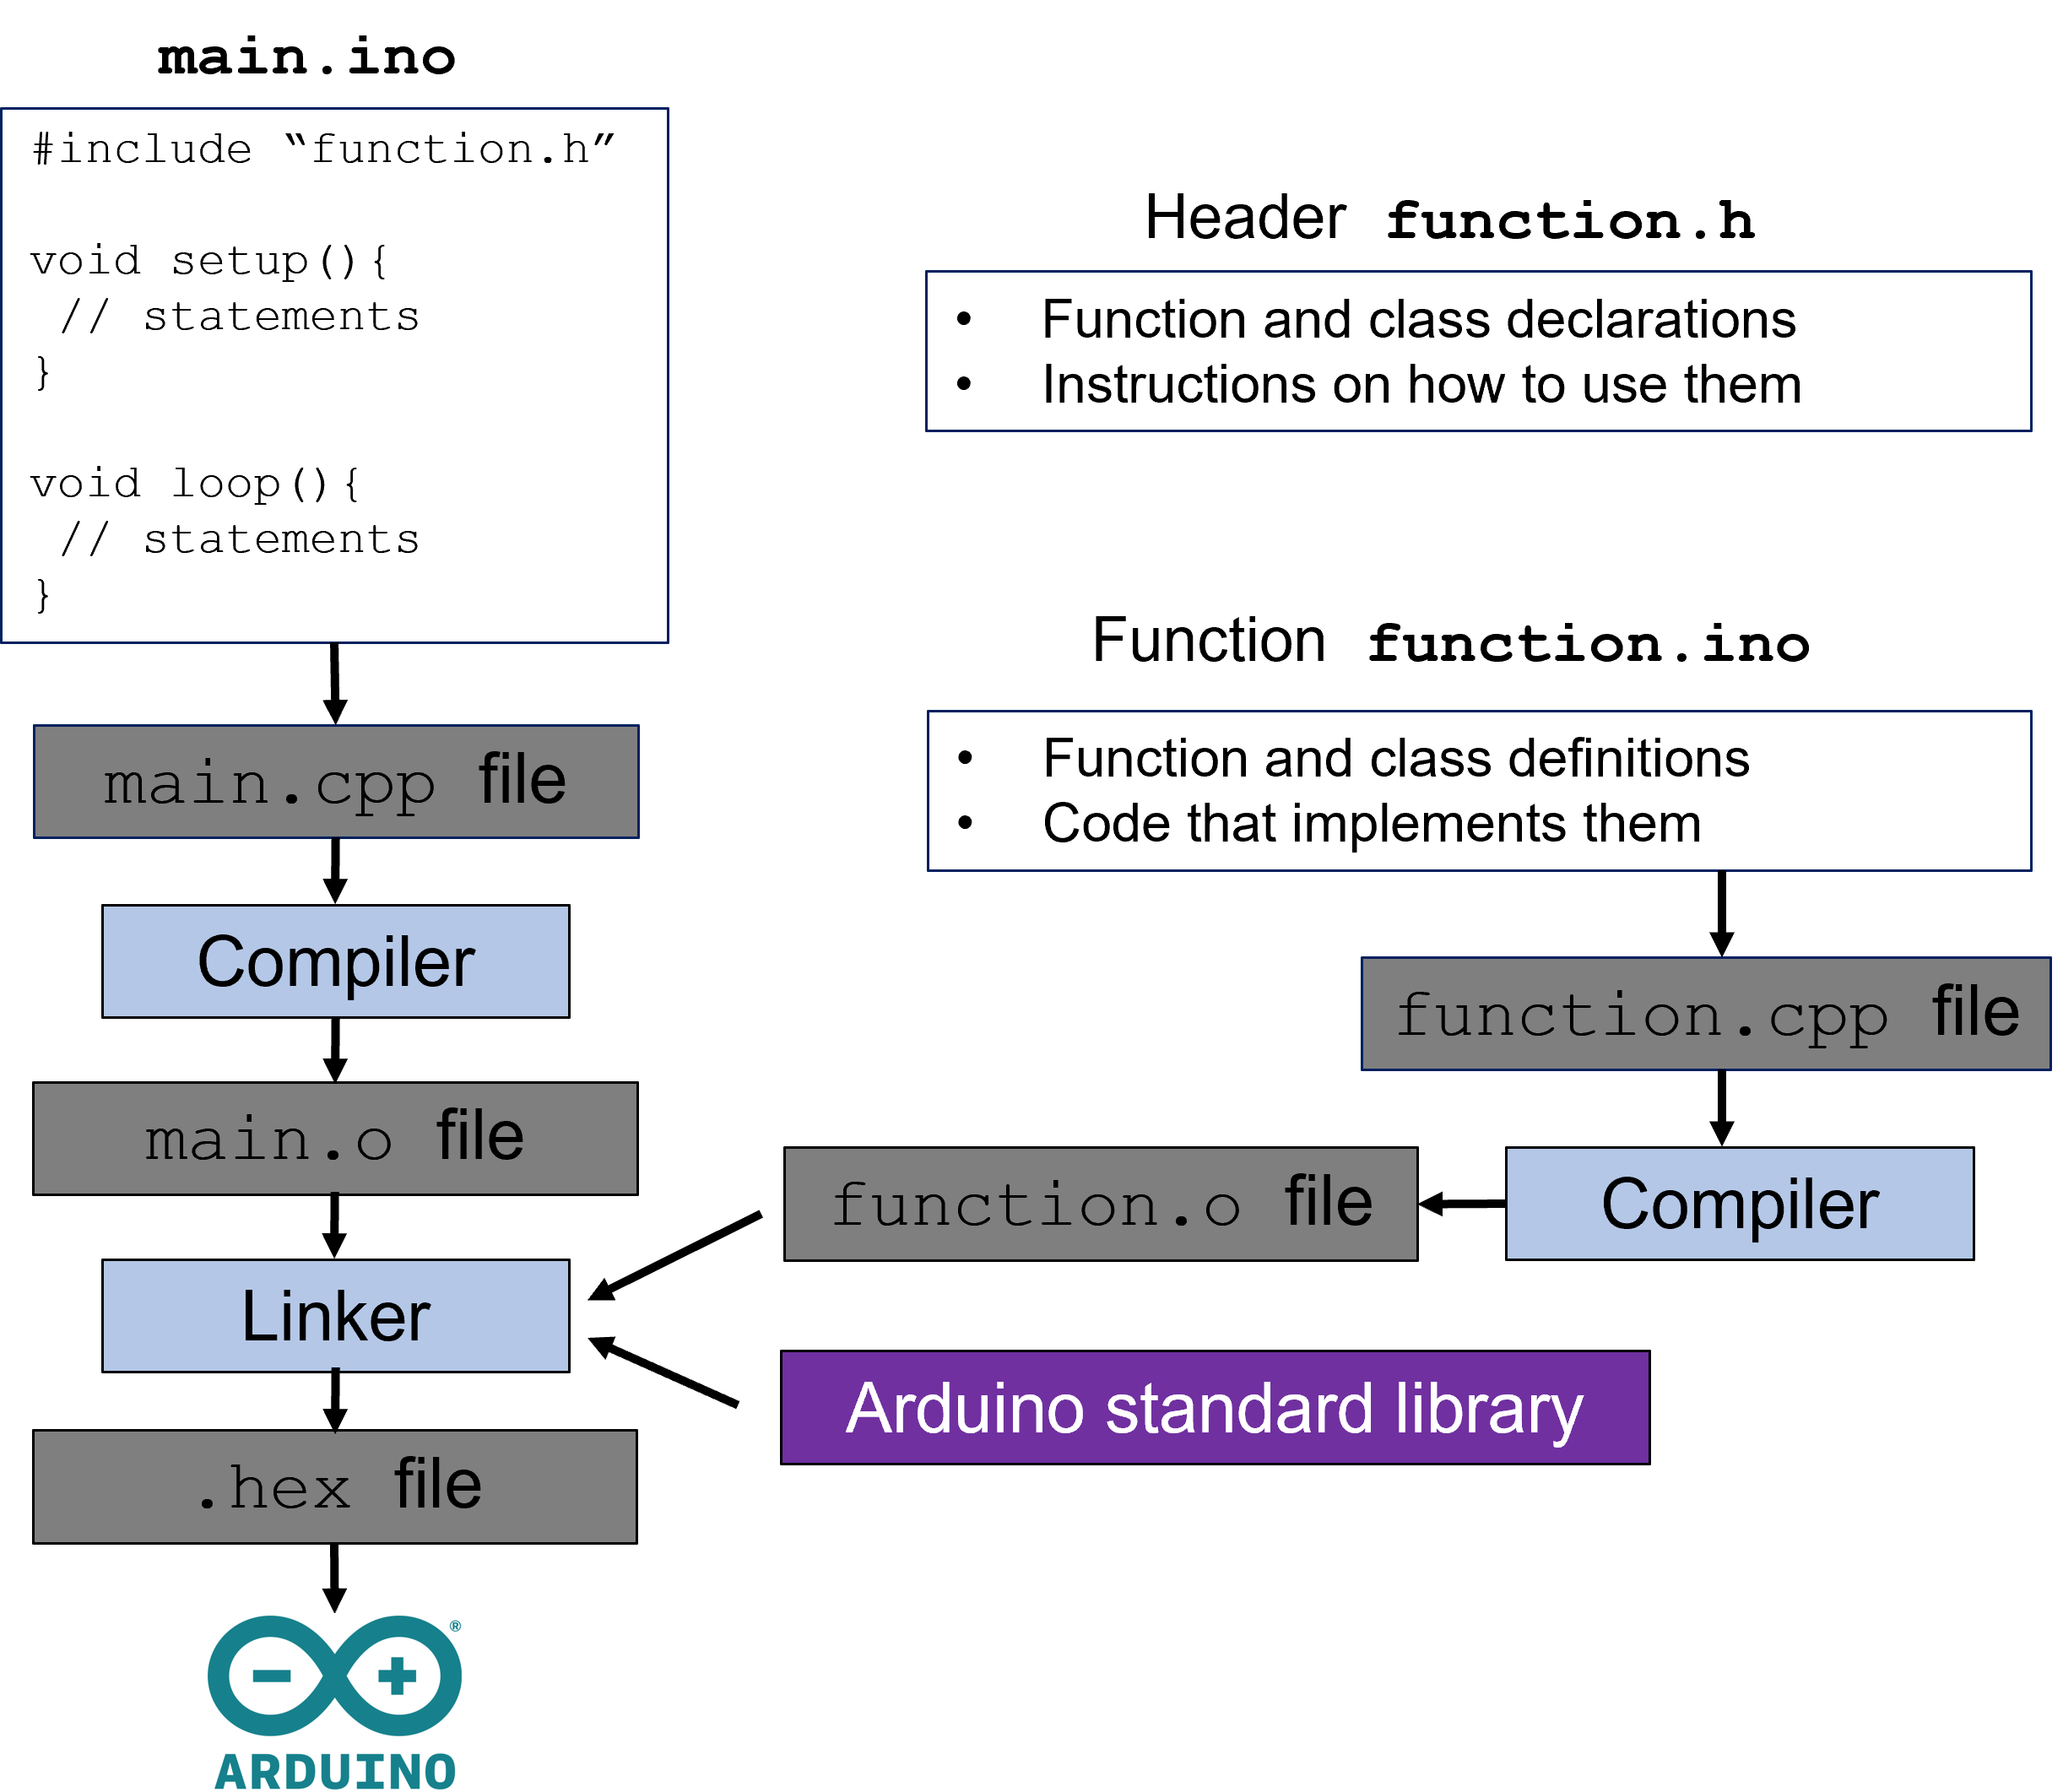
\includegraphics[width=.65\textwidth]{compile.png}
    \caption{Arduino pre-processing, compilation and uploading flowchart}
\end{figure}
\noindent C/C++ language shares a very similar compilation process to the one shown above!

\newpage 
\section{Pointers}
``Wait what...?  Pointers? Point to where?", you may ask. The best answer to this question (ever!) is the formal definition: \textbf{A pointer is a variable that contains the \textit{address} of a variable}. In other words, instead of storing a number or a character, a pointer stores a memory address of another variable. \\\\
Wierd? It should be - this concept isn't found in Python, so you haven't had to work with it before. Let us begin with a simple picture of how memory of your program is organised. A typical machine has an array of consecutively numbered or addressed memory cells. Let us say, 
\begin{itemize}
    \item one cell can hold the memory of one byte - that is, the size of a \texttt{char} variable;
    \item a pair of one-byte cells can be treated as a \texttt{short int} variable;
    \item two pairs of adjacent one-byte cells represent a \texttt{long int} type variable. 
\end{itemize}
A pointer is a group(two or four) of memory cells that can hold an address.
\begin{figure}[H]
    \centering
    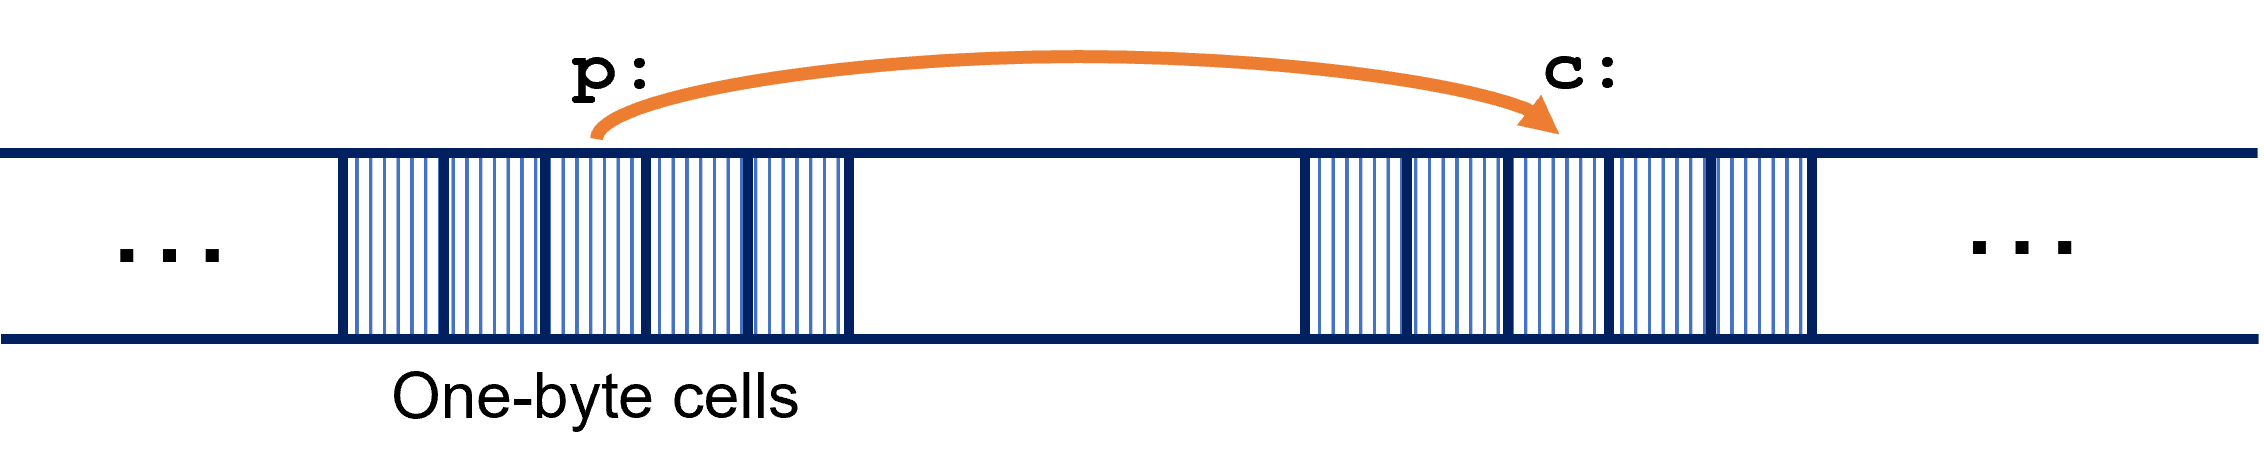
\includegraphics[width=.6\textwidth]{pointer.png}
    \caption{Memory location and pointer}
    \label{fig:pointer}
\end{figure}
\noindent If \texttt{c} is a \texttt{char} type variable, \texttt{p} is a pointer that points to the memory location of \texttt{c}, the situation can be presented in \autoref{fig:pointer}.\\\\
In C and C-like languages, two specific operators, {\Large\textbf{\texttt{\&}}} and {\Large\textbf{\texttt{*}}}, are used to \textbf{reference} and \textbf{dereference} a pointer. 
\begin{enumerate}
    \item The operator {\Large\textbf{\texttt{\&}}} gives the address of an object. 
% do NOT change the indentation
\begin{lstlisting} 
p = &c;
\end{lstlisting}
    \vspace{-.7cm} which assigns the address of \texttt{c} to the variable \texttt{p}, say, ``\texttt{p} points to \texttt{c}''.
    
    \item The operator {\Large\textbf{\texttt{*}}} dereferences the address. When applied to a pointer, it accesses the object the pointer points to.
\begin{lstlisting} 
int *ptr;           // declare a pointer
int a = 1;          // declare a int variable and assign 1 to it
ptr = &a;           // assign the address of `a' to `ptr'
printf("%d", *ptr); // deference the pointer, access to `a'
\end{lstlisting} \vspace{-.7cm}
\noindent The last command \texttt{printf("\%d", *ptr)} prints out the value of the variable \texttt{a} by derefencing the pointer \texttt{ptr}. Note that, \texttt{\%d} in the function \texttt{printf} is a \href{https://www.geeksforgeeks.org/format-specifiers-in-c/}{format specifier} in C language, it just means the data printed is an integer.
\end{enumerate}

\noindent \textbf{Why use pointers?} Firstly, pointers allow functions to change the specific variables sent to them - not copies of the values, but the original memory locations of the variables themselves. This is useful when you are working on a large dataset, for example; you may not have enough memory to make a copy every time you pass the data to a function, but with a pointer, you can work on the data itself, without needing to copy it. Secondly, pointers are used to implement arrays. Especially when working with \href{https://en.wikipedia.org/wiki/C_dynamic_memory_allocation}{dynamic memory allocation}. Thirdly, pointers make code faster - copying large datasets every time you call a function takes time. And finally, pointers are  used in \href{https://en.wikipedia.org/wiki/Object-oriented_programming}{object-oriented programming}.\\\\
\noindent \textbf{Why not use pointers?} Pointers allow you to directly access memory addresses, which makes them very \textbf{dangerous}. If you do not use your pointers correctly you can access garbage data, overwrite important parts of your data or your program itself, or you can leave the pointers dangling. Another product of incorrect usage may be \href{https://en.wikipedia.org/wiki/Memory_leak}{memory leaks}.

% {\color{red}
% \begin{framed}
% \centering The descriptions regarding the pros and cons of pointers are very brief. There is plenty more to learn about them!
% \end{framed}}

\newpage
\section{(A warm-hearted) Checklist}
This is a general checklist generated by Mr Paschal Egan, NOT specifically related to the questions that YOU have encountered. Adapted from \textit{Appendix D, Arduino First-year Task Sheet} (2021).  
\begin{enumerate}
    \item Have you set in tools correct Arduino and com port (highest) – a particular problem with shared computers it is saves last user’s set up.
    \item If the Arduino powered? – Sure? If have a known good/ spare always a good idea to swap.
    \item Is the device being recognized as a USB device? (Look at device manager plugging in and out)
    \item Try another USB port – on some laptops the left-hand side USB ports are USB2 and the right are USB3 and the driver is only installed for one or other.
    \item If you have a Nano which needs the CH340 driver – is it installed? Google how to install the driver if needed – the original nano and the UNO use the FTDI chip whose driver is part of windows.
    \item Regression is a powerful idea. If fails to compile go back to earlier version (even as far as back to “Blink” – if that does not work what has changed since it last did?)
    \item Double check selected correct Arduino version, and correct COM port (generally highest one)
    \item Hardware swap out. Try another PC, another cable, another Arduino. Ideally have a fully working parallel system and bit by bit morph one into the other.
    \item If going on a forum for help, give as much details as possible: version of the IDE, version of the hardware, what operating system used, where the problem is (compiles / but does not load? / device not detected? / does not compile? / unexpected behaviour? etc.)
\end{enumerate}

\vspace{2cm}

\section{Interesting links, fantastic ideas}
\begin{enumerate}
    \item 20 Awesome Arduino UNO Projects: \\
    \href{https://www.seeedstudio.com/blog/2020/01/16/20-awesome-arduino-projects-that-you-must-try-2020/}{https://www.seeedstudio.com/blog/2020/01/16/20-awesome-arduino-projects-that-you-must-try-2020/}\\ {\color{gray}(I love the idea of auto plant watering system so much!)}
    
    \item OKdo Blog - a regularly-updated web for your Arduino project inspirations: \href{https://www.okdo.com/okdo-blog/}{https://www.okdo.com/okdo-blog/}
    
    \item Build your own Arduino from scratch using ATMega328P: \\ \href{https://www.instructables.com/Make-Your-Own-Arduino-ArduinoISP-Learn-to-Burn-Boo/}{https://www.instructables.com/Make-Your-Own-Arduino-ArduinoISP-Learn-to-Burn-Boo/}

\end{enumerate}

\end{appendices}
%%=====================================

\end{document}